\newcommand{\java}{Java 8}
\newcommand{\mavenLarge}{Apache Maven 3.6.3}
\newcommand{\maven}{\texttt{maven} }
\newcommand{\ciglib}{\texttt{CigLib} }
\newcommand{\toml}{\texttt{Toml}}
\newcommand{\dto}{\texttt{DTO} }
\newcommand{\factoryDTO}{\texttt{FactorySMSDatagram} }

\begin{document}
\section{Anàlisis de requisits}
Des d'un punt de vista general, al voler realitzar una simulació, els requisits del projecte no tenen la projecció d'un entorn realista, ja que l'objectiu és dur a terme un anàlisis dels costos empírics del projecte, com per exemple, veure on està el coll d'ampolla o mesurar i poder parametritzar els valors més idonis pel protocol.
\\
\\
En més concret, s'han trobat els següents requisits:
\begin{itemize}
	\item Des del punt de vista d'arquitectura de xarxa, es pot veure clarament que el model es pot definir com client-servidor, ja que la interacció entre les diferents entitats és centralitzada.
	\item És important mantenir el codi el més obert possible per tal de realitzar els canvis de la manera més còmode, sobretot en els següents apartats: la connexió entre els clients i el servidor i la incorporació de diferents criptosistemes per realitzar el xifratge.
	\item S'ha de tenir en consideració el llenguatge i les eines a utilitzar per tal de facilitar la lògica.
	\item S'ha d'intentar tenir la capacitat de realitzar els canvis sobre diferents paquets i llibreries en cas que es necessiti.
	\item Un cop creada la implementació, s'ha de poder realitzar un anàlisis de costs el més detallat possible.
	\item El sistema tant pel punt de vista del comptador com per la subestació ha de ser totalment configurable. És a dir, s'ha de passar per paràmetre la configuració del protocol explicada en la secció \ref{sec:configuracio-recsi}.
\end{itemize}
\subsection{Característiques tècniques}
La simulació del projecte s'ha implementat utilitzant \texttt{\java} i \texttt{\mavenLarge} per la gestió de paquets. Per tal d'executar el projecte, es recomana usar la comanda explícita de \maven:
\begin{verbatim}
mvn exec:java -D exec.mainClass=<main-class>
\end{verbatim}
La classe serà aquella que té el mètode estàtic \texttt{main}, com per exemple:
\begin{verbatim}
	mvn exec:java -Dexec.mainClass=cat.udl.cig.sms.main.NeighborhoodSimulation 
	        -Dexec.args="16"
\end{verbatim}
Pel que fa els tests, la comanda per executar-los és:
\begin{verbatim}
mvn test
\end{verbatim}
La decisió d'utilitzar \texttt{\java} s'ha degut a la llibreria \ciglib creada per Víctor Mateu, que recopila implementacions tant de sistemes criptogràfic com de funcions hash, entre altres. D'aquesta forma, s'intenta assolir el màxim els requisits detallats anteriorment. La implementació del projecte es troba en un repositori remot a GitHub \cite{smart}.
\\
\\
A l'utilitzar \maven per la gestió de paquets i dependència, s'ha canviat l'estructura de la llibreria i s'ha pujat a un repositori remot \cite{ciglib}. Per instal·lar-la només cal configurar el servidor de \texttt{GitHub} a \maven i cridar la dependència des de la configuració del projecte.
\lstset{language=xml}
\begin{lstlisting}
<dependency>
	<groupId>cat.udl.cig</groupId>
	<artifactId>cig-lib</artifactId>
	<version>1.0-SNAPSHOT</version>
</dependency>
\end{lstlisting}
Pel que fa a la configuració del sistema, s'ha decidit utilitzar el format \toml\footnote{Format de fitxer per a fitxers de configuració.} ja que és fàcil i ràpid de llegir i d'escriure a causa de la seva sintaxi i semàntica minimalista i està dissenyat per transformar sense ambigüitats el fitxer a un diccionari.
\section{Disseny}
El projecte es divideix en un total de cinc paquets que s'encarreguen de diferents responsabilitats.
\begin{itemize}
	\item \texttt{connection} s'encarrega d'aportar la connexió entre els comptadors i la subestació, carregant d'aquesta manera els diferents \textit{datagrames} o  \texttt{Data Transfer Objects} (\texttt{DTO}).
	\item A \texttt{busom} hi ha la implementació de \cite{busom}.
	\item \texttt{consumption} es responsabilitza de rebre les lectures de consum d'energia.
	\item A \texttt{recsi} s'hi trobarà la implementació de la proposta \cite{recsi}.
	\item Al paquet \texttt{main} hi ha les diferents classes on s'inicia l'aplicació. \label{list:packages}
\end{itemize}
\subsection{Configuració}
La configuració del sistema i de cada entitat (sigui comptador o subestació ) ve donada per dos fitxers:
\begin{itemize}
	\item Fitxer de configuració del sistema, que serà compartit per totes les entitats del barri, ja que inclourà:
	\begin{itemize}
		\item La corba el·líptica.
		\item El punt generador de la corba.
		\item El cos primer de la corba.
	\end{itemize}
	Les dades d'aquest fitxer estan encapsulades a la classe \texttt{CurveConfiguration}, que funciona com una \texttt{dataclass}\footnote{Classe que només té la responsabilitat d'encapsular informació.}.
	\begin{figure}[H]
		\centering
		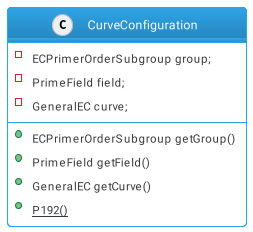
\includegraphics[width=4.5cm]{classes/curve.png}
		\caption{Classe \texttt{CurveConfiguration}}
		\label{fig:curve}
	\end{figure}
	Com es pot veure a la \textit{Figura \ref{fig:curve}}, s'ha creat un mètode estàtic per retornar la configuració de la corba \texttt{P192} de \texttt{NIST} \cite{p192}, la qual és usada per als tests i per l'anàlisis de costos.
	\item Fitxer de configuració de xarxa, on vindrà donada la direcció $ip$ del servidor i el seu port on escolta. D'aquesta manera, la subestació, donada aquesta configuració, crearà un \texttt{ServerSocket} per escoltar en el port i cada comptador crearà un \texttt{Socket} que estarà enllaçat al socket del servidor. S'ha creat mètodes estàtics en la classe \texttt{SocketReader} que realitzaran la lectura del fitxer de configuració i crearan el socket que faci falta.
	\begin{figure}[H]
		\centering
		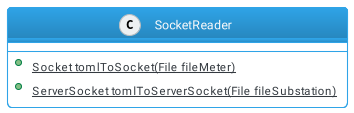
\includegraphics[width=6cm]{classes/socket.png}
		\caption{Classe \texttt{SocketReader}}
		\label{fig:socket}
	\end{figure}
	
\end{itemize}
\subsection{Connexió}
Com que els comptadors i les subestacions no tenen el mateix comportament pel que fa a la connexió, en \texttt{connection} trobem tres interfícies que representen les diferents responsabilitats del paquet:
\begin{itemize}
	\item \texttt{ReceiverMeter }s'encarrega de rebre el \dto de la subestació.
	\item \texttt{ReceiverSubestation }rebrà tots els \dto dels comptadors.
	\item \texttt{Sender} només s'encarregarà d'enviar \dto ja sigui de part d'un comptador o de la subestació.
\end{itemize}
Aquestes interfícies corresponen, en un cert grau, a l'arquitectura de client servidor, per aquest motiu, la forma més fàcil d'implementar la lògica era creant un servidor per la subestació i un client pel comptador.
La implementació s'ha realitzat usant les classes \texttt{Socket} i \texttt{ServerSocket} de \texttt{java.net} pels comptadors i la subestació respectivament.
\begin{figure}[H]
	\centering
	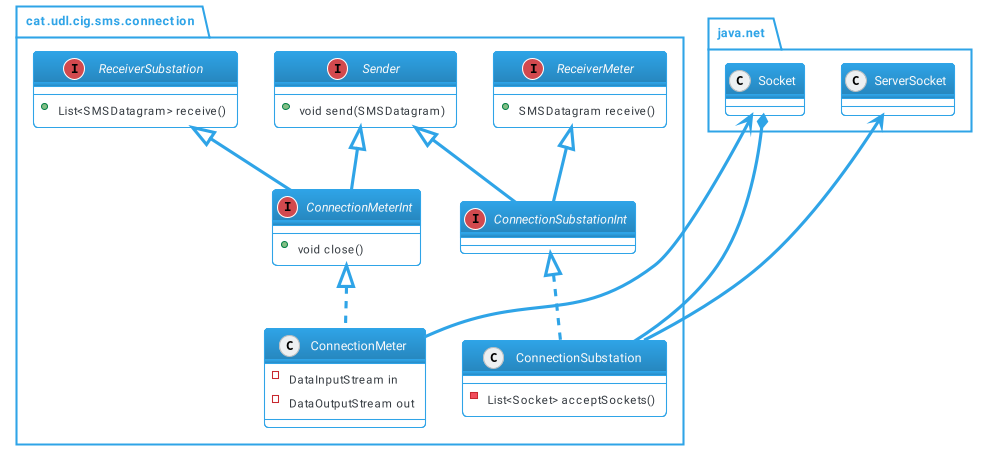
\includegraphics[width=16cm]{classes/connection.png}
	\caption{Diagrama de classe del paquet connection}
	\label{fig:connection}
\end{figure}
\subsubsection{Data Transfer Objects}
Al haver de realitzar enviaments amb diferent contingut, s'han creat cinc datagrames, tal i com es pot observar a la \textit{Figura \ref{fig:dto}}. En cada una de les classes s'ha usat el patró \textit{factory method}, creant la interfície \texttt{SMSDatagram}, per serialitzar-los a la nostra manera.
\begin{figure}[H]
	\centering
	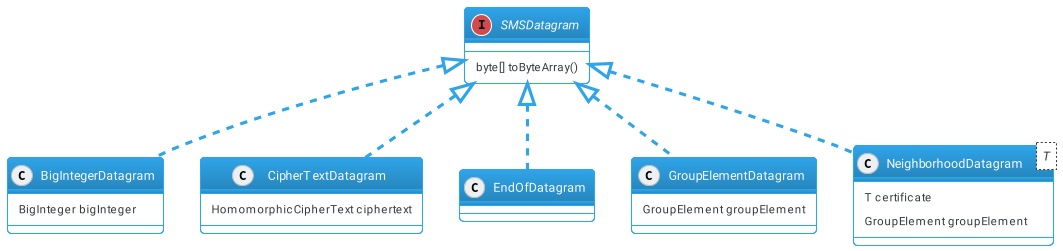
\includegraphics[width=16cm]{classes/dto.png}
	\caption{Diagrama de classe dels DTO}
	\label{fig:dto}
\end{figure}
A més a més, en algun moment voldrem desserialitzar-los, és a dir, donat un vector de bytes, obtenir un objecte de la classe \texttt{SMSDatagram}. Com que \texttt{\java } no soporta interfícies o classes abstractes amb mètodes estàtics per definir, s'ha creat una altra interfície anomenada \texttt{SMSDatagramSerializer} amb el mètode \texttt{fromBytes} les implementacions la qual retornaran un \texttt{SMSDatagram}. Amb l'objectiu de saber quin serialitzador usar en cada cas només sabent l'array de bytes, s'ha creat la classe \texttt{SerializerRepository}, un \textit{singleton} que contindrà totes les serialitzacions i, usant el mètode \texttt{buildDatagramFromInput} retornarà el datagrama que correspongui.
\begin{figure}[H]
	\centering
	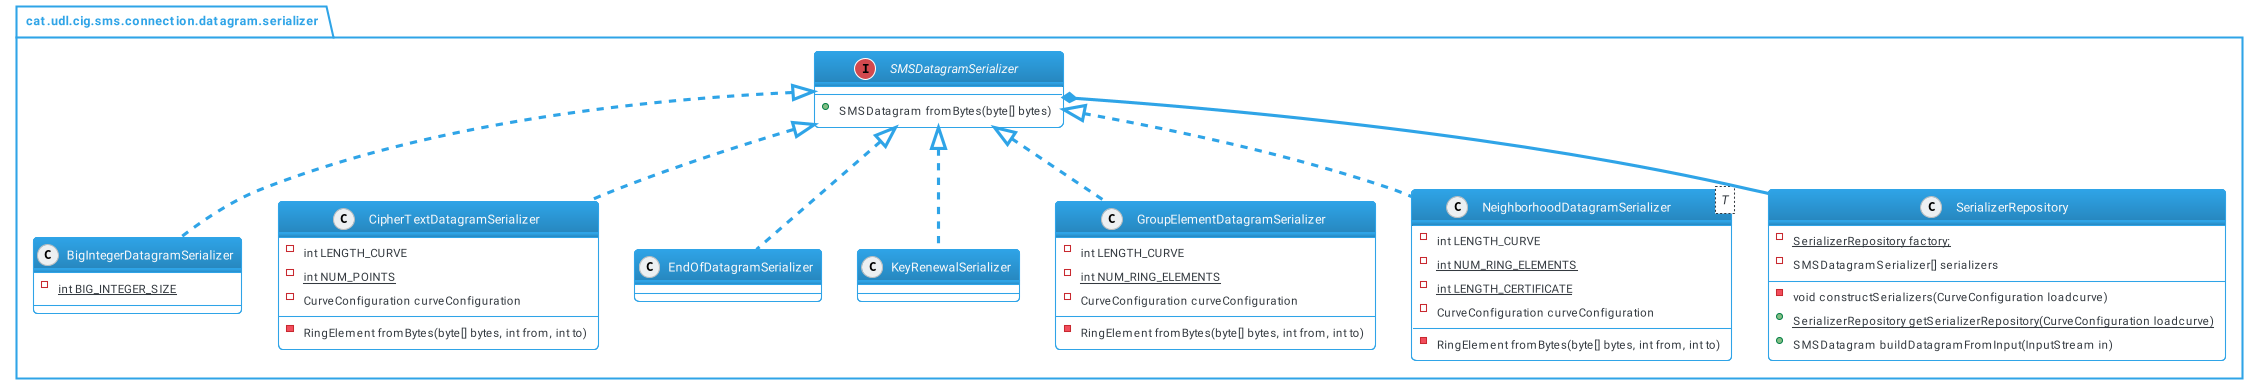
\includegraphics[width=16cm]{classes/dtoser.png}
	\caption{Diagrama de classe dels serialitzadors de DTO}
	\label{fig:dtoser}
\end{figure}


\subsection{Criptografia}
A l'hora de fer una primera iteració sobre el projecte, es va decidir crear una capa entre \ciglib i el sistema, d'aquesta manera, s'intenta satisfer el requisit de mantenir el codi el més obert possible per a possibles futurs canvis. Per exemple, en el cas de voler usar un altre criptosistema homomòrfic per passar les claus de manera xifrada, només caldria que aquest heretés de \texttt{HomomorphicCypher} i usar-lo en \texttt{DecryptChunk}. Un altre cas interessant és també mantenir el més obert a extensions l'algoritme per calcular el logaritme discret, on només s'hauria de crear una classe de \texttt{LogarithmAlgorithm}. Tal i com es pot veure a la \textit{Figura \ref{fig:logarithm}}, a la llibreria \cite{ciglib} s'ha implementat tres classes que hereden d'ella, entre elles, \textit{Pollard's Lambda}.
\begin{figure}[H]
	\centering
	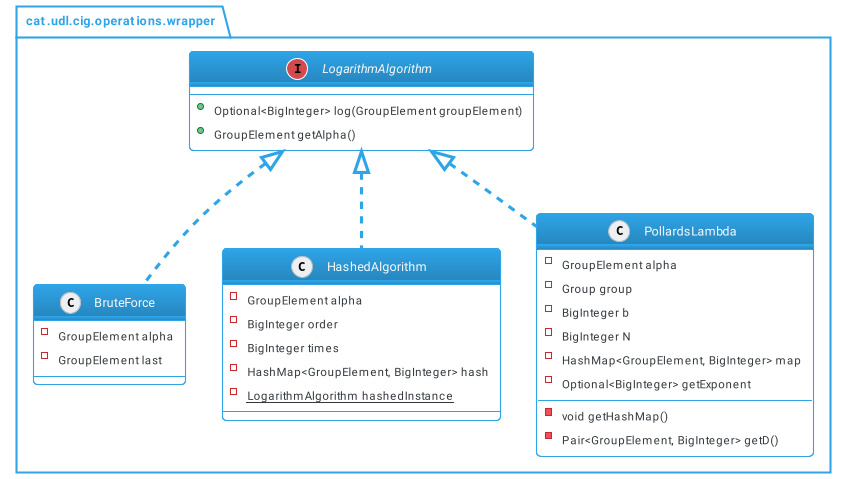
\includegraphics[width=16cm]{classes/log.png}
	\caption{Diagrama de classe LogarithmAlgorithm}
	\label{fig:logarithm}
\end{figure}
A l'hora de crear \texttt{PollardsLambda}, es va solventar un error que no permetia crear una funció \textit{Hash} correctament, a causa de com estava implementat el mètode \texttt{hashcode} de la classe \texttt{GroupElement} de \cite{ciglib}. Per tal d'avançar la implementació, es va crear l'algoritme \texttt{BruteForce} per usar-lo en els tests i en fases més inicials del projecte, quan encara no estava implementat el \texttt{PollardsLambda}. Més endavant, es va idear \texttt{HashedAlgorithm}. Aquesta classe està dissenyada com un \texttt{Singleton}, on primer es realitza un algoritme de força bruta per guardar tots els valors del logaritme discret de qualsevol element. D'aquesta manera, el mètode solament haurà d'accedir a memòria i serà l'únic cost. Al igual que \texttt{PollardsLambda}, aquest mètode depèn del \texttt{hashcode} de \texttt{GroupElement}, per tant, es necessitava tenir solventat l'error també per aquesta implementació. A causa d'això, es va realitzar una correcció general per totes les classes de \cite{ciglib}.
\subsection{Patró Màquina-Estat}
Per tal de crear una lectura entenedora dins de la complexitat del protocol, es va pensar en implementar-lo utilitzant el patró de disseny \texttt{Màquina-Estat}. L'avantatge d'utilitzar aquesta arquitectura de disseny davant de les altres és l'analogia que comparteix amb diagrames de flux o d'estat, cosa que permet implementar algoritmes complexos de manera més senzilla. \texttt{Màquina-Estat} resumeix tota la lògica relativa als estats i a les transicions, és a dir, ens podrem estalviar condicionals i problemes de complexitat de lectura en el codi.
\\
\\
Aquest patró consisteix en tenir una interfície \textit{Estat} amb el mètode \textit{next}, que retornarà el nou \textit{Estat} donat el context de l'aplicació. És important tenir en consideració que el treball a realitzar dels comptadors i de la subestació serà diferent i, per tant, la implementació dels estats no es compartirà. D'aquesta manera, el punt o estat del programa estarà determinat pels tipus d'\textit{Estat} que estan la subestació i els comptadors en aquell moment. Gràcies a això, creant unes validacions i precondicions adequades, la màquina d’estat impedeix operacions fora del nostre entorn.
\\
\\
No obstant això, aquest tipus d'arquitectura també té inconvenients. Un d'ells és que la seva rigidesa impedeix crear una bona estructura per projectes que necessiten molta asincronia. Per sort, el nostre protocol és el suficientment rígid per no necessitar accions d'asincronia, és més, la implementació es quedarà beneficiada d'aquesta rigidesa. Com que els comptadors hauran d'anar sincronitzats en cada ronda, la subestació no haurà de tenir diferents estats segons l'estat de cada comptador ni la seva informació específica referent a això, sinó que es relaxarà el problema tenint un estat global relacionat a tots els comptadors.
\newpage
\subsubsection{Implementació en \cite{recsi}}
Tant la subestació com els comptadors comparteixen el nombre d'estats del protocol, que corresponen a la fase d'establiment de claus i configuració i la fase de la transmissió del consum, tal i com es pot veure a la \textit{Figura \ref{fig:recsi-state}}.
\begin{figure}[H]
	\centering
	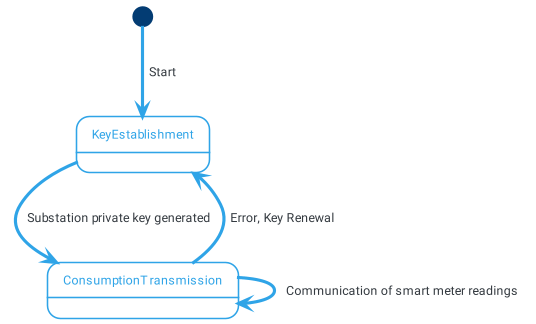
\includegraphics[width=7cm]{classes/recsistate.png}
	\caption{Màquina d'estats del protocol \cite{recsi}}
	\label{fig:recsi-state}
\end{figure}
En relació a la implementació, en el paquet \texttt{recsi}, es troben dos interfícies:
\begin{itemize}
	\item \texttt{SubstationStateContextInt}, que es responsabilitza de començar la coumicació i l'establiment de claus i realitzar la transferència de les lectures de manera segura i agregada.
	\item \texttt{State}, on cada extensió es responsabilitzarà de cada acció que ha de fer en el pas que toqui.
\end{itemize}
A la \textit{Figura \ref{fig:recsi}} es troben dos implementacions de \texttt{State} que corresponen a les dos fases del protocol respectivament. A més a més, es pot veure que \texttt{SubstationStateContext} conté tant la configuració de la corba, la connexió, com el possible missatge rebut que correspondrà a l'última transmissió de les lectures. Addicionalment, aquesta classe serà qui instanciarà els estats. Per això mateix, els estats necessiten tenir la referència del context i \texttt{State} i \texttt{SubstationStateContext} tenen una relació de composició. 
\begin{figure}[H]
	\centering
	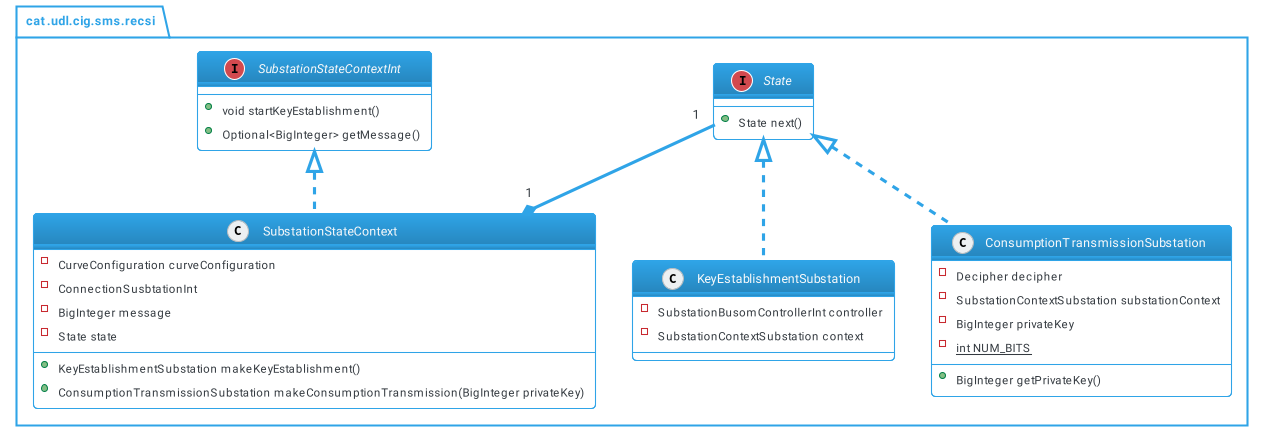
\includegraphics[width=16cm]{classes/recsi.png}
	\caption{Diagrama de classe dels estats de la subestació}
	\label{fig:recsi}
\end{figure}
\subsubsection{Implementació en \cite{busom}}
La implementació del protocol de \cite{busom} segueix un disseny molt semblant, creant un context per tal de guardar l'estat en cada moment del protocol. A més a més, per tal deixar obert a possibles noves implementacions o variants del protocol de comunicació de configuració s'han creat les interfícies \texttt{MeterBusomServiceInt} i \texttt{SubstationBusomServiceInt}, les implementacions les quals es responsabilitzen de cridar la implementació del protocol i d'enviar la clau privada en divisions, en el cas dels comptadors, i de computar la clau privada, en el cas de la subestació. El nombre de paquets a transmetre estan en la configuració de \texttt{KeyEstablishmentMeter} en el cas dels comptadors, ja que és responsabilitat de \cite{recsi} dividir la clau privada en fragments, i \texttt{SubstationBusomService} en el cas de la subestació, ja que és el servei el qui ha de controlar la transmissió \cite{busom}.
\\
\\
Cal esmentar que existeixen mètodes \texttt{protected} en la implementació del protocol que no apareixen a la \textit{Figura \ref{fig:diss-busom}}, ja que aquests només són usats i han de ser usats en tests.
\begin{figure}[H]
	\centering
	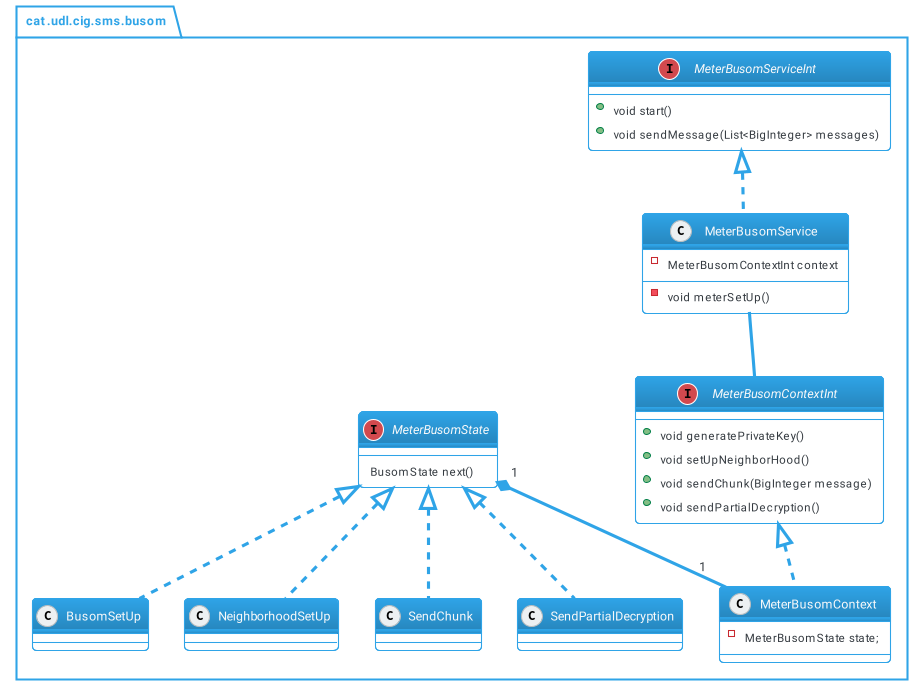
\includegraphics[width=14cm]{classes/busomprot.png}
	\caption{Diagrama de classe dels estats dels comptadors.}
	\label{fig:diss-busom}
\end{figure}
Com es pot veure a les \textit{Figures \ref{fig:busom-state}} i  \textit{\ref{fig:busom-state-sub}}, a la màquina d'estats del comptador se li ha afegit un estat de més, aquest sent \textit{BusomSetUp}, on només genera la clau privada. Es podria prescindir d'aquesta deicisió d'implementació i afegir-ho en la responsabilitat de \textit{NeighborhoodSetUp}, però es va creure oportú fer-ho així per dos motius:
\begin{itemize}
	\item tenir les tasques el més dividides i estructurades possibles. 
	\item poder prescindir de la sincronia amb la subestació per tal de realitzar tasques que no requerissin una comunicació, com és el cas de la generació de la clau privada de cada comptador.
\end{itemize}
Amb la intenció de tractar i veure què es considera error i què es una clau de renovació, s'ha creat l'excepció \texttt{KeyRenewalException}
\begin{figure}[H]
	\centering
	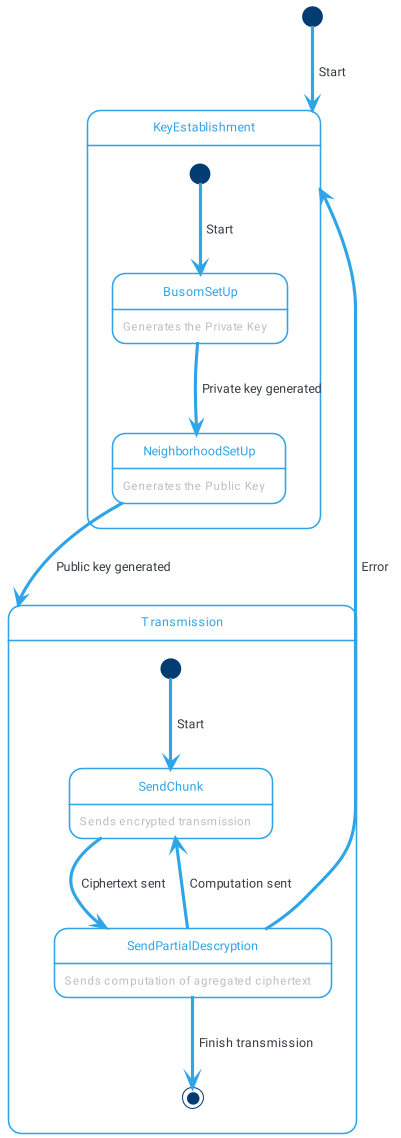
\includegraphics[width=6.5cm]{classes/busomstatemeter.png}
	\caption{Màquina d'estats del protocol \cite{busom}}
	\label{fig:busom-state}
\end{figure}
\begin{figure}[H]
	\centering
	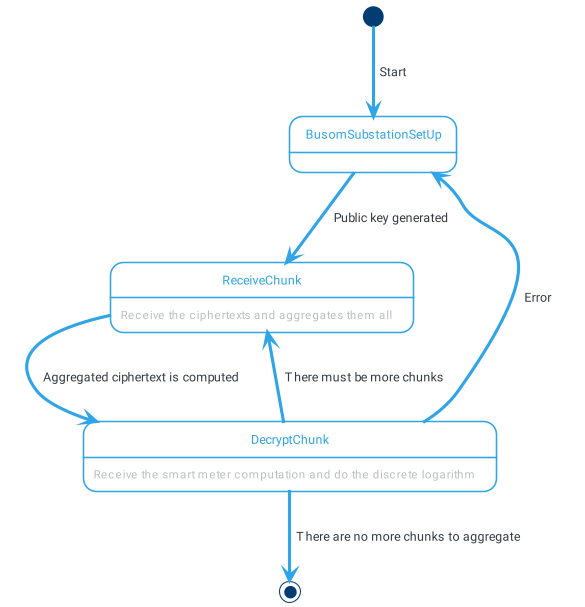
\includegraphics[width=10cm]{classes/busomstatesub.png}
	\caption{Màquina d'estats del protocol \cite{busom}}
	\label{fig:busom-state-sub}
\end{figure}
\subsection{Execució de les simulacions}
En un primer instant, es van crear les classes \texttt{SmartMeterRunnable} i \texttt{SubstationRunnable}, que agafaven la configuració per línea de commandes d'aquesta manera:
\begin{verbatim}
	mvn exec:java -Dexec.mainClass=cat.udl.cig.sms.main.SmartMeterRunnable
	        -Dexec.args="<idMeter> <substationFileName> [<numMsgs>]"
\end{verbatim}
En cas que no s'especifiqui el nombre de missatges a enviar, s'usarà el consum de \texttt{ConsumptionFileReader}, sent el nombre de missatges 92.
\begin{verbatim}
	mvn exec:java -Dexec.mainClass=cat.udl.cig.sms.main.SubstationRunnable 
	        -Dexec.args="<substationFileName> <numMeters> [<numMsgs>]"
\end{verbatim}
No obstant això, es va veure més còmode realitzar una classe que executés per ella mateixa els comptadors i la subestació de manera paral·lela amb l'ús de \textit{threads}.
\begin{verbatim}
mvn exec:java -Dexec.mainClass=cat.udl.cig.sms.main.NeighborhoodSimulation 
       -Dexec.args="<numMeters> [numMsgs]"
\end{verbatim}
A més a més, com que està implementat el protocol \cite{busom} per l'establiment de claus de \cite{recsi}. S'ha pogut adaptar el codi per tal de poder executar el protocol \cite{busom} simulant un sistema de comptadors intel·ligents. Pel que fa a les classes d'execució, es segueix la mateixa estructura que en les classes anteriors, de manera que podem executar la subestació o els comptadors per si sols o generar tota la comunitat.
\begin{verbatim}
mvn exec:java -Dexec.mainClass=cat.udl.cig.sms.main.busom.BusomMeterRunnable
       -Dexec.args="<idMeter> <substationFileName> [<numMsgs>]"
\end{verbatim}
De la mateixa forma que en el cas anterior,  si no s'especifica el nombre de missatges a enviar, s'usarà el consum de \texttt{ConsumptionFileReader}, on el nombre de missatges és 92.
\begin{verbatim}
mvn exec:java -Dexec.mainClass=cat.udl.cig.sms.main.busom.BusomSubstationRunnable 
       -Dexec.args="<numMeters> [<numMsgs>]"
\end{verbatim}
\begin{verbatim}
mvn exec:java -Dexec.mainClass=cat.udl.cig.sms.main.busom.BusomNeighborhood
       -Dexec.args="<numMeters> [numMsgs]"
\end{verbatim}
\end{document}
